\documentclass[smallheadings]{scrartcl}

%%% GENERAL PACKAGES %%%%%%%%%%%%%%%%%%%%%%%%%%%%%%%%%%%%%%%%%%%%%%%%%%%%%%%%%%
% inputenc allows the usage of non-ascii characters in the LaTeX source code
\usepackage[utf8]{inputenc}
\usepackage{graphicx}


% title of the document
\title{LGS mit LU Zerlegung}
% optional subtitle
%\subtitle{Draft from~\today}
% information about the author
\author{%
 Aron Ventura und Annika Thiele\\ Humboldt-Universit\"at zu Berlin
}
\date{\today}


%%% LANGUAGE %%%%%%%%%%%%%%%%%%%%%%%%%%%%%%%%%%%%%%%%%%%%%%%%%%%%%%%%%%%%%%%%%%
% babel provides hyphenation patterns and translations of keywords like 'table
% of contents'
\usepackage[ngerman]{babel}

\usepackage{amsthm}
\newtheorem{theorem}{Satz}


\theoremstyle{definition}
\newtheorem{definition}{Definition}[section]


%%% HYPERLINKS %%%%%%%%%%%%%%%%%%%%%%%%%%%%%%%%%%%%%%%%%%%%%%%%%%%%%%%%%%%%%%%%
% automatic generation of hyperlinks for references and URIs
\usepackage{hyperref}

%%% MATH %%%%%%%%%%%%%%%%%%%%%%%%%%%%%%%%%%%%%%%%%%%%%%%%%%%%%%%%%%%%%%%%%%%%%%
% amsmath provides commands for type-setting mathematical formulas
\usepackage{amsmath}
% amssymb provides additional symbols
\usepackage{amssymb}
% HINT
% Use http://detexify.kirelabs.org/classify.html to find unknown symbols!

%%% COLORS %%%%%%%%%%%%%%%%%%%%%%%%%%%%%%%%%%%%%%%%%%%%%%%%%%%%%%%%%%%%%%%%%%%%
% define own colors and use colored text
\usepackage[pdftex,svgnames,hyperref]{xcolor}

%%% nice tables
\usepackage{booktabs}

%%% Code Listings %%%%%%%%%%%%%%%%
% provides commands for including code (python, latex, ...)
\usepackage{listings}
\definecolor{keywords}{RGB}{255,0,90}
\definecolor{comments}{RGB}{0,0,113}
\definecolor{red}{RGB}{160,0,0}
\definecolor{green}{RGB}{0,150,0}
\lstset{language=Python, 
        basicstyle=\ttfamily\small, 
        keywordstyle=\color{keywords},
        commentstyle=\color{comments},
        stringstyle=\color{red},
        showstringspaces=false,
        identifierstyle=\color{green},
        }

\usepackage{graphicx}
\usepackage{paralist}

\usepackage[style=authoryear, backend=biber,natbib=true]{biblatex}
\addbibresource{LU}

% setting the font style for input und returns in description items
\newcommand{\initem}[2]{\item[\hspace{0.5em} {\normalfont\ttfamily{#1}} {\normalfont\itshape{(#2)}\/}]}
\newcommand{\outitem}[1]{\item[\hspace{0.5em} \normalfont\itshape{(#1)}\/]}
\newcommand{\bfpara}[1]{
	
	\noindent \textbf{#1:}\,}

\begin{document}

% generating the title page
\maketitle
\newpage
% generating the table of contents (requires to run pdflatex twice!)
\tableofcontents
\newpage

%%% BEGIN OF CONTENT %%%%%%%%%%%%%%%%%%%%%%%%%%%%%%%%%%%%%%%%%%%%%%%%%%%%%%%%%%

\section{Einf\"uhrung in die Theorie}
	\subsection{Motivation und Problemstellung}
Das Poisson Problem findet in vielen Anwendungsbereichen wie zum Beispiel der Elektrostatik, der Hydrostatik, der Gravitation und der Wärmeleitung Anwendung.
	 	Das motiviert, sich mit dem numerischen Lösen des Differentialgleichungssystems auseinander zu setzen. Man kann das Problem diskretisieren und erhält so ein lineares Gleichungssystem, welches wir dann mithilfe der sogenannten $LU$ Zerlegung lösen. Es stellt sich die Frage, wie effizient und genau man eine Lösung finden kann. Deshalb schauen wir uns in diesem Bericht mit zunehmender Feinheit der Diskretisierung den Fehler, aber auch die Sparsität, sowie Kondition der Matrix des Gleichungssystems an. 


	\subsection{Theoretischer Hintergrund}
		\subsubsection{Poisson Problem}
		Wir definieren den Laplace Operator wie in \citep{PDE}.
		\begin{definition}[Laplace Operator]
		Der Laplace Operator einer Funktion $u\in C^2(\mathbb{R}^d,\mathbb{R})$ ist definiert durch
		$$\Delta u=\sum_{i=1}^d\frac{\partial ^2 u}{\partial x_i^2}$$

		\end{definition}
		Wir definieren weiter das partielle Differentialgleichungssystem wie in \citep{PDE}, welches im Poisson-Problem gelöst werden soll. Wir betrachten das Problem auf einem  Gebiet  $\Omega$ und Rand $\partial \Omega$. seien $f\in C(\Omega , \mathbb{R})$ und $g\in C(\partial \Omega , \mathbb{R})$ Funktionen. Dann suchen wir eine Funktion $u$, sodass
		\begin{align*}
		\Delta u&=f \text{ in }\Omega\\
		u&= g \text{ auf }\partial\Omega
		\end{align*}
		WIr betrachten in diesem Bericht einen Spezialfall des Problems, wo $\Omega =(0,1)^d$, $d\in \{1,2,3\}$ und $g\equiv 0$

		Wir wollen das Problem numerisch mit \textit{Finiten-Differenzen} approximieren. Nach \citep{finite}
		\begin{definition}[Finite-Differenzen-Methode]
		Finite-Differenzen-Methoden sind eine Klasse numerischer Verfahren zur Lösung gewöhnlicher und partieller Differenzialgleichunen.		
		Die grundlegende Idee bei der \textit{Finite-Differenzen-Methode} ist es die Ortsableitung in der Differenzialgleichung an einer endlichen Zahl Gitterpunkten durch Differenzenquotienten zu approximieren. Unsere angenäherten Lösungen der Differenzialgleichung an den Gitterpunkten führen dann auf ein entsprechendes Gleichungssystem, welches sich numerisch berechnen lässt.
		\end{definition}
		In unserem Fall diskretisieren wir dazu das Gebiet $\Omega$ und den Laplace Operator durch \textit{Finite Differenzen} um ein lineares Gleichungssystem zu erhalten.
		 Im Folgenden wird die Theorie hinter unserem Verfahren zum numerischen lösen des Problems nach \citep{PDE}, \citep{Wiki}. Wir diskretisieren das Gebiet indem wir das Intervall $(0,1)$ in $n$ äquidistante Teilintervalle zerlegen. Die so entstehenden Gitterpunkte im $(0,1)^d$ werden unsere Diskretisierungspunkte. Mit den Finiten Differenzen zweiter Ordnung können wir den Laplace Operator diskretiseren, denn wir wissen aus \citep{Wiki}, dass 
		$$\frac{\delta^2u}{\delta x_l^2} \approx D_h^{(2)} u_{x,l}(x) =\frac{u(x_1,...,x_l+h,...,x_d) - 2u(x_1,...,x_l,...,x_d) + u(x_1,...,x_l-h,...,x_d)}{h^2}$$
		gilt. 
		Um ein lineares Gleichungssystem zu erhalten, definieren wir eine Ordnung auf den Diskretisierungspunkten.
		\begin{definition}
		Seien $x=(x_1,...,x_d)$ und $y=(y_1,...,y_d)$ zwei Diskretisierungspunkte. Dann gilt $x <_X y$ genau dann, wenn
		$$\sum_{l=1}^dx_ln^l<\sum_{l=1}^dy_ln^l$$
		\end{definition}
		Sei $N:=(n-1)^d$ die Anzahl an Diskretisierungspunkten.
		So erhalten wir $N$ lineare Gleichungen und damit Blockmatrizen $A^{(d)}$, für die zu lösen gilt $A^{(d)}\hat{u}=b$. Wir definieren diese Blockmatrizen induktiv.
		$$A^{(d)}_{1} := \begin{pmatrix}     2d & -1 & 0 & 0 &\dots&0 \\    -1 & 2d & -1 & 0&\dots&0 \\    0&\ddots&\ddots&\ddots&\ddots&\vdots\\    \vdots & \ddots &\ddots&\ddots&-1&0 \\    0 & \dots&0&-1&2d&-1\\     0&  \dots&0&0&-1&2d    \end{pmatrix}$$
		$$A^{(d)}_{l} := \begin{pmatrix}     A^{(d)}_{l-1} & -\mathbf{I}_{l-1} & 0 & 0 &\dots&0 \\    -\mathbf{I}_{l-1} & A^{(d)}_{l-1} & -\mathbf{I}_{l-1} & 0&\dots&0 \\    0&\ddots&\ddots&\ddots&\ddots&\vdots\\    \vdots & \ddots &\ddots&\ddots&-\mathbf{I}_{l-1}&0 \\    0 & \dots&0&-\mathbf{I}_{l-1}&A^{(d)}_{l-1}&-\mathbf{I}_{l-1}\\     0&  \dots&0&0&-\mathbf{I}_{l-1}&A^{(d)}_{l-1}    \end{pmatrix}$$
		Wir setzen $A^{(d)}:=A^{(d)}_d$ Die rechte Seite $b$ erhalten wir durch das Einsetzen der Diskretisierungspunkte in die gegebene Funktion $f$. 

		\subsubsection{Kondition und Sparsität einer Matrix}
		Wir betrachten ein mathematisches Problem $P(x)=y$. Dann interessiert uns, wie sich eine Störung oder ein relativer Fehler im Input $\frac{||\Delta x||}{||x||}$ sich im Output fortpflanzt. Dies motiviert die Definition der relativen Kondition wie in \citep{Skript}.
				\begin{definition}[(relative) Kondition]
		Die (relative) Kondition eines Problems $P$ ist der kleinste Faktor $K$ mit der Eigenschaft, dass für alle Inputdaten $x$ und für alle Outputdaten $y$ gilt 
		$$\frac{||\Delta y||}{||y||}\leq K\frac{||\Delta x||}{||x||}$$
		\end{definition}
		\begin{definition}[Kondition einer Matrix]
		Die Kondition einer Matrix $A$ ist definiert durch $\text{cond}(A):=||A||\cdot ||A^{-1}||$
		\end{definition}
		Die Kondition dieser Matrix enstspricht der relativen Kondition des Problems $Ax=b$, gibt also ein Maß an, wie sich der Fehler beim Lösen eines Linearen Gleichungssystems verhält. 

		Wir betrachten die Matrizen $A^{(d)} \in \text{Mat}(\mathbb{R}^{(n-1)^d},\mathbb{R}^{(n-1)^d})$. Die Anzahl der Einträge wird also mit wachsender Feinheit, also wachsendem $n$ sehr schnell groß. Allerdings sind nur einige Einträge ungleich Null. Wir sprechen wie in \citep{PDE} von \textit{sparse}, also dünnbesetzte Matrizen. Betrachtet man den Speicherbedarf einer solchen Matrix kann es also sinnvoll sein, statt die Matrix intuitiv als Array von Arrays abzuspeichern, die nicht-null Einträge und deren Position zu speichern. 

Wir werden in unseren Experimenten die Kondition von Hilbertmatrizen betrachten. Dazu definieren wir an dieser Stelle:
		\begin{definition}[Hilbertmatrix]
		Die Hilbert Matrix der Ordnung $n$ ist definiert als 
		$$\begin{pmatrix}
		1&\frac{1}{2}&\frac{1}{3}&\cdots & \frac{1}{n}\\
		\frac{1}{2}&\frac{1}{3}&\frac{1}{4}&\cdots &\frac{1}{n+1}\\
		\frac{1}{3}&\frac{1}{4}&\frac{1}{5}&\cdots &\frac{1}{n+2}\\
		\vdots &\vdots &\vdots &\ddots &\vdots\\
		\frac{1}{n}&\frac{1}{n+1}&\frac{1}{n+2}&\cdots &\frac{1}{2n-1}\\
		\end{pmatrix}$$
		\end{definition}
		
		\subsubsection{Lösen eines Gleichungssystems mit der LU Zerlegung}
	In der Linearen Algebra haben wir bereits zum Lösen von Gleichunssystemen den Gaußschen Algorithmus kennengelernt. Beim Durchführen des Gaußschen Algorithmus an eine Matrix $A$ wird diese Matrix in eine  oberen rechten Dreiecksmatrix mit Einsen auf der Hauptdiagonalen und einer unteren linken Dreicksmatrix zerlegt. Eine solche Zerlegung nennt man auch \textit{LU-Zerlegung}. Die Theorie hinter der $LU$ ZERlegung ist in Anlehnung an \citep{Skript}.
	\begin{definition}[LU-Zerlegung]
	Eine Zerlegung einer Matrix $A$ der Form $A=L\cdot U$ mit einer unteren linken Dreiecksmatrix mit Einsen auf der Hauptdiagonalen $L$ und eine oberen rechten Dreiecksmatrix $U$:
	\begin{align*}
	L=\begin{pmatrix}
	1&0&\cdots&0&0\\
	*&1&\cdots&0&0\\
	\vdots&\vdots&\ddots&\vdots&\vdots\\
	*&*&\cdots&0&0\\
	*&*&\cdots&*&1
	\end{pmatrix},
	U=\begin{pmatrix}
	*&*&\cdots&*&*\\
	0&*&\cdots&*&*\\
\vdots&\vdots&\ddots&\vdots&\vdots\\
	0&0&\cdots&*&*\\
	0&0&\cdots&0&*
	\end{pmatrix}
	\end{align*}
	heißt \textit{LU-Zerlegung}.
	\end{definition}
	\begin{theorem}
	Jede reguläre Matrix lässt sich LU-zerlegen mit 
	$$PA=LU$$
	wobei $P$ eine geeignete Permutationsmatrix ist. 
	\end{theorem}
	\begin{proof}
	Sei $A$ eine reguläre Matrix $A=(a_{i,j})$. Wir setzten $A^{(0)}:=A$. Dann gilt für $$L_1=\begin{pmatrix}
	
	1&0&\cdots&0&0\\
	-l_{21}&1&\cdots&0&0\\
	\vdots&\vdots&\ddots&\vdots&\vdots\\
	-l_{n2}&0&\cdots&0&1

	\end{pmatrix}	
	$$ mit $l_{i1}=\frac{a_{i1}^{(0)}}{a_{11}^{(0)}}$, dass
$$A^{(1)}:=L_1\cdot A^{(0)}$$ gilt mit 
$$A^{(1)}=\begin{pmatrix}
a_{11}^{(1)}&a_{12}^{(1)}&\cdots &a_{1n}^{(1)}\\
0&a_{22}^{(1)}&\cdots &a_{2n}^{(1)}\\
\vdots&\vdots&\ddots&\vdots\\
0&a_{n2}^{(1)}&\cdots & a_{nn}^{(1)}
\end{pmatrix}
	$$
	Im $i$-ten Schritt des Gauss-Algorithmus erhalten wir
	$$ A^{(i)} = L_iA^{(i-1)}$$
	mit
	$$ A^{(i)}=\begin{pmatrix}
	a_{11}^{(i)}&a_{12}^{(i)}&\cdots&a_{1i}^{(i)}&a_{1,i+1}^{(i)}&\cdots&a_{1n}^{(i)}\\
	0&a_{22}^{(i)}&\cdots&a_{2i}^{(i)}&a_{2,i+1}^{(i)}&\cdots&a_{2n}^{(i)}\\
	\vdots&\vdots&\ddots&\vdots&\vdots&&\vdots\\
	0&0&\cdots&a_{ii}^{(i)}&a_{i,i+1}^{(i)}&\cdots&a_{in}^{(i)}\\
	0&0&\cdots&0&a_{i+1,i+1}^{(i)}&\cdots&a_{i+1,n}^{(i)}\\
	\vdots&\vdots&&\vdots&\vdots&\ddots&\vdots\\
	0&0&\cdots&0&a_{n,i+1}^{(i)}&\cdots&a_{nn}^{(i)}
	\end{pmatrix}
	$$
	und $$L_1:=\begin{pmatrix}
	1&\cdots&0&0&0&\cdots&0\\
	\vdots&\ddots&\vdots&\vdots&\vdots&&\vdots\\
	0&\cdots&1&0&0&\cdots&0\\
	0&\cdots&0&1&0&\cdots&0\\
	0&\cdots&0&-l_{i+1,i}&1&\cdots&0\\
	\vdots&&\vdots&\vdots&\vdots&\ddots&\vdots\\
	0&\cdots&0&-l_{n,i}&0&\cdots&1\\
	\end{pmatrix}
	$$wobei $$l_{k,i}:=\frac{a_{k,i}^{(i-1)}}{a_{i,i}^{(i-1)}}$$
	Nach $n-1$ Schritten erhalten wir dann insgesamt
	$$A^{(n-1)}=L_{n-1}A^{(n-2)}=\cdots=L_{n-1}L_{n-2}\cdots L_{1}A^{(0)}\\$$
	und damit
	$$L_{1}^{-1}L_{2}^{-1}\cdots L_{n-1}^{-1}A^{(n-1)}=A^{(0)}$$
	Hierbei ist $$U:=A^{(n-1)}$$ eine obere Dreiecksmatrix und es lässt sich leicht nachrechnen, dass $$L:=L_{1}^{-1}L_{2}^{-1}\cdots L_{n-1}^{-1}=\begin{pmatrix}
	1&0&\cdots&0&0\\
	l_{21}&1&\cdots&0&0\\
	\vdots&\vdots&\ddots&\vdots&\vdots\\
	l_{n-1,1}&l_{n-1,2}&\cdots&1&0\\
	l_{n1}&l_{n2}&\cdots&l_{n,n-1}&1
	\end{pmatrix}
	$$ eine untere Dreiecksmatrix mit Einsen auf der Hauptdiagonalen ist.
	Damit haben wir schon unsere Zerlegung $$LU=A$$
	\end{proof}		
	
	\subsubsection{Pivotisierung}
	Um zu verhindern, dass beim Invertieren große Einträge in der $L$-Matrix stehen, die eventuell andere Einträge \textit{auslöscht} wollen wir die Matrizen $L_i$, die im $i$-ten Schritt des Gauss-Verfahrens entstehen, so wählen dass die \textit{Kondition} minimal wird.
	Für die \textit{Kondition} gilt:
	\begin{align*}
	cond_1(L_i)&=||L_i^{-1}||_1||L_i||_1\\
	&=\left(1+\sum_{k=i+1}^{m}|l_{ki}|\right)^2\\
	&=\left(1+\sum_{k=i+1}^{m}\left|\frac{a_{ki}^{(i-1)}}{a_{ii}^{(i-1)}}\right|\right)^2
	\end{align*}
	Wir wollen im $i$-ten Eliminationsschritt also unser \textit{Pivotelement} $a_{ii}$ möglichst groß
	wählen.
	
	Sei also $k^*$ so, dass
	$$ |a_{k^*i}^{(i-1)}|= \max_{k=1,...,n} |a_{ki}^{(i-1)}|$$
	
	Dazu tauschen wir die $i$-te Zeile mit der $k^*$-ten Zeile.
	Hierzu verwenden wir die Matrix $P$, die aus der Einheitsmatrix entsteht indem man die $i$-te und $k^*$-te Spalte tauscht.
	$$P_i=\begin{array}{cc}
	\begin{array}{c}
	\begin{pmatrix}	
	1&0&\cdots&0&\cdots&0&\cdots&0&0\\
	0&1&\cdots&0&\cdots&0&\cdots&0&0\\
	&&\ddots&\vdots&&\vdots&&&\\
	&&&0&&1&&&\\
	\vdots&\vdots&&\vdots&\ddots&\vdots&&\vdots&\vdots\\
	&&&1&&0&&&\\
	&&&\vdots&&\vdots&\ddots&&\\
	0&0&\cdots&0&\cdots&0&\cdots&1&0\\
	0&0&\cdots&0&\cdots&0&\cdots&0&1
	\end{pmatrix}
	\end{array}&\begin{array}{cc}
	&\\
	&\\
	&\\
	\leftarrow&i\text{-te Zeile}\\
	\\
	\leftarrow&k^*\text{-te Zeile}\\
	&\\
	&\\
	&\\
	\end{array}
	\end{array}	
	$$	
	
	Damit finden wir $$A^{(i)}=L_iP_iA^{(i-1)}$$ wobei $L_i$ optimal konditioniert ist.
	
	Wir erhalten also nach dem $(n-1)$-ten Eliminationsschritt.
	$$A^{(n-1)}=L_{n-1}P_{n-1}L_{n-2}P_{n-2}\cdots L_{1}P_{1}A^{(0)}$$

	Da $P_i$ jeweils sein eigenes Inverses ist, können wir folgendermaßen mit der Einheitsmatrix multiplizieren:
	$$A^{(n-1)}=L_{n-1}P_{n-1}L_{n-2}P_{n-2}\cdots L_{2}P_{2}L_{1}P_{2}P_{2}P_{1}A^{(0)}$$
	Man kann leicht sehen, dass $P_{2}L_{1}P_{2}=L_{1}$ gilt, und somit 
$$A^{(n-1)}=L_{n-1}P_{n-1}L_{n-2}P_{n-2}\cdots L_{2}L_{1}P_{2}P_{1}A^{(0)}.$$
Induktiv können wir so alle Permutationsmatrizen an den $L$ Matrizen vorbeischieben, sodass wir folgende Gleichung erhalten.
$$A^{(n-1)}=L_{n-1}L_{n-2}\cdots L_{1}P_{n-1}P_{n-2}\cdots P_{1}A^{(0)}.$$


	
	Mit $$L:=L_{1}^{-1}L_{2}^{-1}\cdots L_{n-1}^{-1}$$
	und $$P:=P_{n-1}P_{n-2}\cdots P_1$$ und $$A^{(n-1)}=U$$
	erhalten wir $$PA=LU$$
	
	
\section{Implementierung}
\subsubsection*{Bedienungshilfe \texttt{block\_matrix.py}}
In \texttt{block\_matrix.py} ist eine \texttt{main()} Funktion implementiert. Sie dient zur Demonstration ausgewählter vorhandender Funktionen und
		wird nur ausgef\"uhrt wenn \texttt{block\_matrix.py} direkt mittels \texttt{python3 experiments\_lu.py} gestartet wird. 
Anschließend hat der Nutzer die Möglichkeit einen von zwei Graphen einzusehen. Auch hier gibt es eine Exception bei einem \texttt{ValueError}.
Nach Eingabe von '0' wird ein Plot erstellt, der die Kondition in Abhängigkeit von $N$ zeigt. Betrachtet werden bis zu $595$ Diskretisierungspunkte und 1 bis 3 Dimensionen. 
Wird jedoch '1' eingegeben, so wird ein Plot zu den selben $N$ dargestellt, jedoch wird dann die Anzahl an Nicht-Null-Einträgen für Dimension $d=1,2,3$ verglichen.
\subsubsection*{Bedienungshilfe \texttt{linear\_solvers.py}}In \texttt{linear\_solvers.py} ist eine \texttt{main()} Funktion implementiert. Sie dient zur Demonstration ausgewählter vorhandender Funktionen und
		wird nur ausgef\"uhrt wenn \texttt{linear\_solvers.py} direkt mittels \texttt{python3 experiments\_lu.py} gestartet wird. 
Anschließend stellt das Programm die Funktionalität von \texttt{solve\_lu()} vor. Zunächst wird zu einer gegebenen $LU$ Zerlegung und rechten Seite das Gleichungssystem gelöst.
Es wird die LU-Zerlegung für eine Koeffizienenmatrix $A$ mit gegebenen Werten $n$, $d$  erstellt. Standardmäßig sind $n=5$ und $d=2$ ausgewählt, aber das kann leicht im Programm geändert werden. Zu beachten ist, dass $n\geq 2$ und $d\geq 1$ sein muss. und in \texttt{block\_matrix.get\_lu()} eingesetzt. Um für $b$ ein Array in der passenden Form zu erhalten nehmen wir $[1,2,\cdots,(n-1)^d]$.
Das Programm gibt dann die Lösung $x$ zur Gleichung $Ax=b$ aus.
	

\subsection{Bedienungshilfe \texttt{experiments\_lu.py}}
In \texttt{experiments\_lu.py} ist eine \texttt{main()} Funktion implementiert. Sie dient zur Ausf\"uhrung der 
		betrachtenten Experimente und
		wird nur ausgef\"uhrt wenn \texttt{experiments\_lu.py} direkt mittels \texttt{python3 experiments\_lu.py} gestartet wird. 
		Nach dem Starten des Programms darf der Benutzende zuerst für \textit{Kappa} eine natürliche Zahl $\geq 100$ ausw\"ahlen. Als nächstes wählt er, welches der Experimente er oder sie sehen möchte. Dazu werden die möglichen Experimente aufgelistet, zusammen mit einer Zahl. Die zugehörige Zahl zum Experiment, das gesehen werden soll, muss danach eingegeben werden. Wird eine andere Eingabe eingegeben, wird der Nutzer darauf hingewiesen und nochmal um eine Eingabe gebeten. Nach dem Auswählen eines Experimentes, wird dieses durchgeführt.
Wird bei einer der Eingaben kein \textit{Integer} angegeben wird eine \texttt{ValueError}-Exception geworfen.\\
\\

\bfpara{\textit{1: Graph zum Fehler der Approximation}}\\
Es wird ein Plot betrachtet der für Dimension $=1,2,3$ den Fehler in Abhängigkeit von $N$ betrachtet. Wir betrachten bis zu $(30-1)^3$ Diskretisierungspunkte.
\bfpara{\textit{2: Vergleich zu Kondition von Hilbertmatrizen}}\\
Es wird schön nebeneinander die Konditionen ausgegeben für Koeffizientenmatrizen mit $1 \leq n \leq  ,1\leq d \leq 3$ und der entsprechenden Hilbertmatrix des selben Formats.
\bfpara{\textit{3: 3D-Graph zur Approximation der Lösung des Poisson-Problems}}\\
Wir stellen graphisch die Exakte Lösung des \textit{Poisson-Problems} für $d=2$ dar, sowie die Approximationen für $n=4,11$.

\bfpara{\textit{4: Vergleich der Sparsity vor und nach LU-Zerlegung}}\\
Hier wird die Anzahl Nicht-Null-Einträge der Koeffizientenmatrizen mit $1 \leq n \leq  ,1\leq d \leq 3$ und die der korrespondierenden LU-Zerlegung einander gegenüber gestellt.
		

\section{Beschreibung der Experimente und Beobachtungen}
Im Rahmen unserer Experimente werden wir uns mit folgender Funktion beschäftigen.
Für $\kappa \in \mathbb{N}$ sei $u:\Omega\rightarrow \mathbb{R}$ definiert durch
$$u(x):=\prod_{l=1}^dx_l\sin (\kappa\pi x_l)$$
Wir berechnen

$$f(x)=\Delta u= \sum_{i=1}^d\frac{\partial ^2 u}{\partial x_i^2}=
 \sum_{i=1}^d \left(\prod_{l\neq i}x_l\sin (\kappa\pi x_l)\right)\left(-x_i\kappa ^2\pi ^2\sin (\kappa\pi x_i)+(1+\kappa\pi)\cos (\kappa\pi x_i) \right)$$

Dann ist $u$ die exakte Lösung zum Poisson Problem mit $f$ wie oben definiert. Wir können also nun numerisch das Poisson Problem lösen und das Ergebnis mit $u$ vergleichen um den Fehler zu erhalten. 

\subsection{Fehleranalyse}

Wir betrachten für die Dimensionen $d\in\{1,2,3\}$ die diskrete Lösung der Poisson-Gleichung für verschiedene Anzahlen an Teilintervallen $n$. Vorallem die Funktion \texttt{get\_sparse()} benötigt mit zunehmendem $n$ sehr schnell sehr lange. So benötigt das Berechnen der Lösung für $d=3$ und $n=25$, also für $13824$ Diskretisierungspunkte bereits $49.41795992851257$ Sekunden. Für $d=2$ und $n=120$, also $14161$ Diskretisierungspunkte $42.58699893951416$ Sekunden. 
Wir wollen uns nun mit dem Fehler der approximierten Lösung beschäftigen. In der folgenden Abbildung ist der Fehler für die verschiedenen Dimensionen in Abhängigkeit von der Anzahl von Diskretisierungspunkten für $\kappa =3$ abgebildet.



\begin{minipage}{\textwidth}

 \centering
 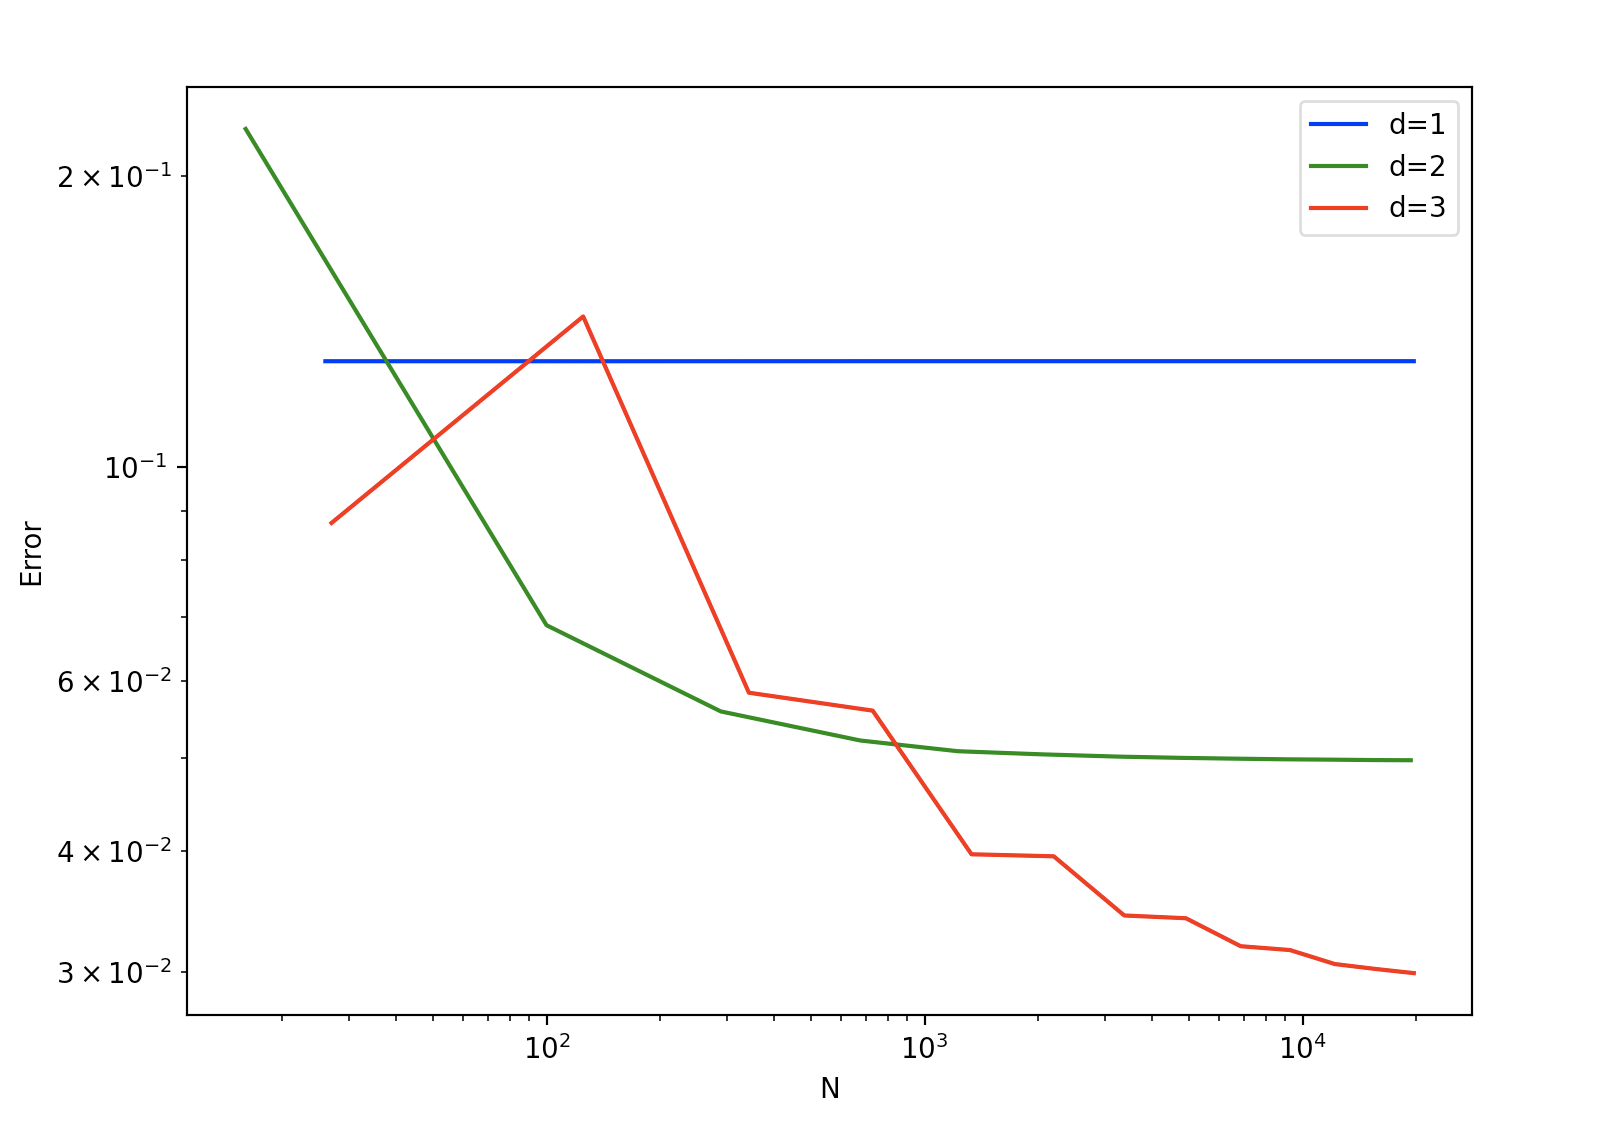
\includegraphics[scale = 0.4]{error}
 	\captionof{figure}{Fehlergraph}
 	\label{error}

 \end{minipage}

 Es lässt sich erkennen, dass der Fehler in der ersten Dimension am größten ist und auch am wenigsten sinkt. In der zweiten dimension sinkt der Fehlergraph anfänglich sehr stark und dann genauso wie in der ersten Dimension. Letzlich sinkt der Fehler in der dritten Dimension am meisten. 

Um genauer die Fortpflanzung des Rundungsfehlers zu untersuchen, addieren wir einen Rundungsfehler $10^{-m}r$ wobei $m$ eine natürliche Zahl ist unr $r$ eine zufällige Zahl zwischen $-\frac{1}{2}$ und $\frac{1}{2}$ ist. Für $\kappa =10$, $m=4$, $n=200$ ist noch kein bemerkenswerter Unterschied zu sehen, aber für $m=3$ sieht der Graph der approximierten Lösung aus wie in Abbildung \ref{conderror} im Anhang. 
Die approximierte Funktion weicht sehr stark von der exakten Funktion $u$ ab. Schaut man sich dieselbe Abbildung mit größeren addierten Fehlern an, so erkennt man, dass die Abweichung immer mehr einer Parabel ähnelt. Dieses Phänomen könnte man  weiterführend untersuchen.

\subsection{Kondition der Blockmatrizen}

Um zu verstehen, wie der Fehler zustande kommt, schauen wir uns nun die Kondition der Blockmatrizen an. Dazu ist in der folgenden Grafik \ref{cond} die Kondition der Matrix in Abhängigkeit von der Anzahl an  Diskretisierungspunkten dargestellt. Die Skalen sind doppelt logarithmisch. 


\begin{minipage}{\textwidth}
\centering
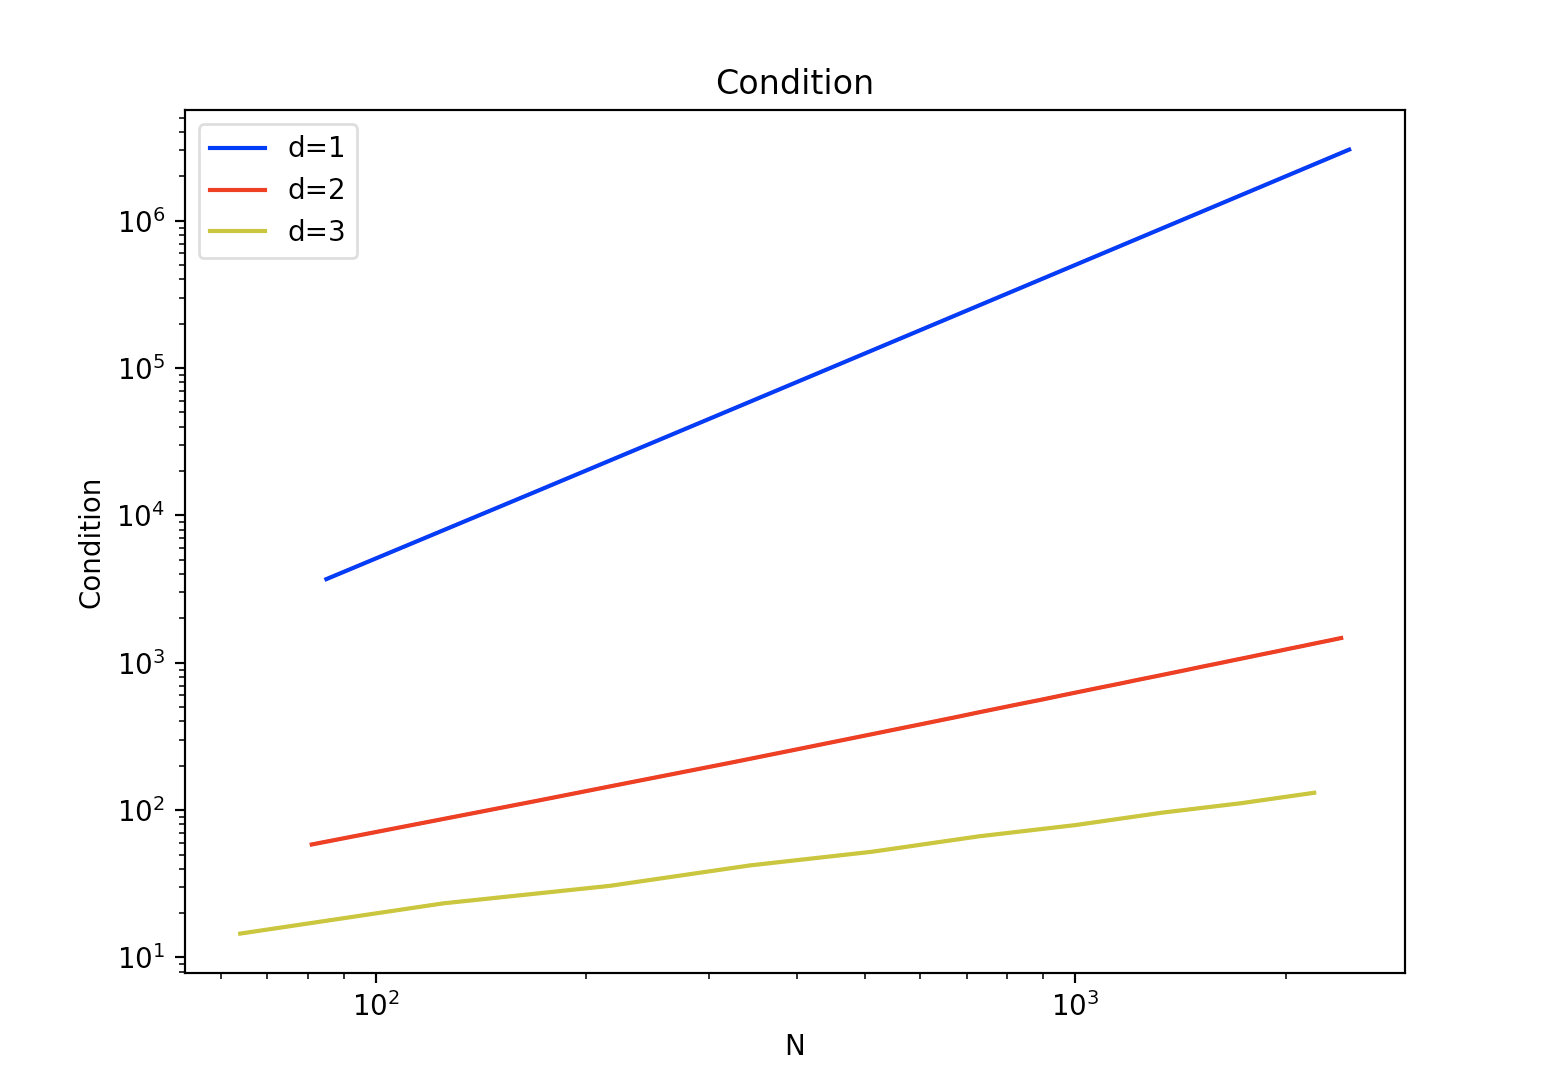
\includegraphics[scale = 0.4]{Condition}
    \captionof{figure}{Kondition der Block Matrizen}
    	\label{cond}
\end{minipage}

Die gelbe Gerade zeigt die Kondition in Abhängigkeit von $N$ für die Dimension $d=3$, die gelbe für $d=2$ und schließlich die blaue für $d=1$. Man kann erkennen, dass die Kondition also exponentiell mit $N$ wächst. Dabei wächst sie aber für niedrige Dimensionen schneller an.

Um die Kondition von den Blockmatrizen in Bezug zu setzen, vergleichen wir sie mit der Kondition von Hilbertmatrizen. In der folgenden Tabelle sind für verschiedene $n$ und $d$ die Kondition von der zugehörigen Blockmatrix und die der Hilbertmatrix der Größe $(n-1)^d$ angegeben. 


\begin{minipage}{\textwidth}
\centering

		\begin{tabular}{c|c|c|c}
			$n$ & \text{Dimension} & \text{Kondition von} $A^{(d)}$ & \text{Kondition von} $H_{(n-1)^d}$\\
			\hline		
			\hline	
			3 & 1 & 3.0 & 27.0\\
			\hline
			4 & 1 & 8.0& 748.0 \\
			\hline
			5 & 1 & 11.999999999999998& 28374.999999999996\\
			\hline
			6 & 1 & 17.999999999999996& 943656.0\\
			\hline
			7 & 1 & 23.999999999999996 &29070278.9999999966 \\
			\hline
			3 & 2 & 3.0 &28374.9999999999964\\
			\hline
			4& 2 & 8.999999999999996 & 1099654541342.59 \\
			\hline
			5 & 2 & 13.333333333333334 & 5.062774787508321e+2216 \\
			\hline
			6&2 & 20.769230769230763 & 2.7744613640462164e+3625 \\
			\hline
			7 & 2 & 27.448275862068975 & 1.7462247118839097e+5336\\
			\hline
			3& 3& 3.0000000000000004& 33872791094.9999968 \\
			\hline
			4 & 3& 9.882352941176471 & 3.069327740892257e+3927\\
			\hline
			5 &3& 14.526315789473685&1.0957826974904638e+9664\\
			\hline
			6 &3& 23.313131313131308 & 2.235417938871472e+189125 \\
			\hline
		
		\end{tabular}
		\captionof{table}{Vergleich Kondition}
		\label{Tabelle}
	\end{minipage}
	Es ist zu erkennen, dass besonders in der dritten Dimension, die Kondition der Hilbertmatrix viel schneller wächst.
	\subsection{Exakte und Approximierte Lösung}
Im Folgenden werden wir die exakte Lösung des Gleichungsystems zusammen mit der approxierten Lösung plotten. Zunächst betrachten wir den eindimensionalen Fall. Die Abbildung \ref{graph()} im Anhang zeigt die genaue und zwei approximierten Lösungen des Problems.




Die blaue gestrichelte Linie zeigt die exakte Lösung des Poisson-Problems. Die blaue durchgezogene Linie stellt die approximierte Lösung für $n=100$, also für $99$ innere Diskretisierungspunkte dar. Letztlich ist die rote Linie die approximierte Lösung für $9$ Punkte. Es ist zu erkennen, dass die blaue durchgezogene Linie schon viel näher an dem eigentlichen Ergebnis ist. Wir betrachten nun den zweidimensionalen Fall. 

Für ein großes $\kappa =100$ sieht derselbe Graph kann man in der Abbildung \ref{bigkappa} im Anhang sehen. Es ist zu erkennen, dass für größere $\kappa$ ein größeres $n$ notwendig ist, um eine halbwegs gute Approximation zu erhalten.


\begin{minipage}{\textwidth}
\centering
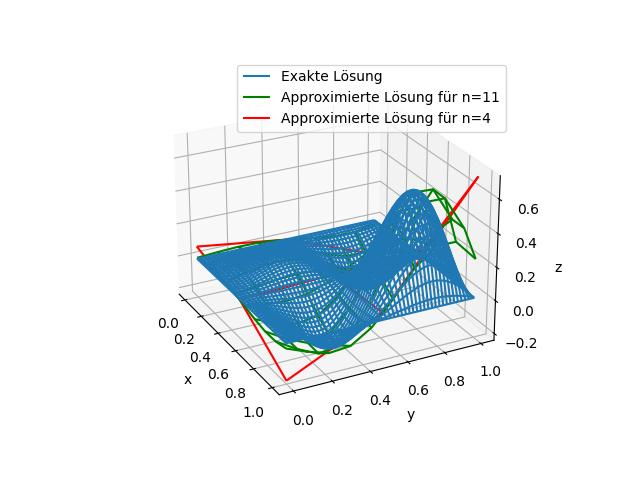
\includegraphics[scale = 0.6]{3D}
	\captionof{figure}{Vergleich exakte und approximierte Lösung für $d=2$}
	\label{3d}
\end{minipage}
In dieser Abbildung zeigt die blaue Funktion den Graphen der Funkton $u(x,y)$, während die rote Funktion die approximierte Lösung an neun Diskretisierungspunkten und die grüne Funktion die approximierte Lösung an $100$ Diskretisierungspunkten darstellt. Auch hier ist zu erkennen, dass die grüne Funktion schon viel näher an der exakten Lösung ist als die rote.



\subsection{Sparsität der LU Zerlegung}

Wir haben schon in der Theorie bemerkt, dass die Blockmatrizen zwar sehr schnell sehr groß werden, aber nur einige Einträge ungleich Null sind. Es handelt sich also um dünnbesetzte Matrizen. Interessant ist nun, wie sie die Sparsität der $LU$ Zerlegung verhält. Dazu ist in der folgenden Abbildung \ref{spar} die Anzahl an Nicht-Null EInträgen von der $LU$ Zerlegung der Blockmatrix in Abhängigkeit von $N$ für die Dimensionen $d\in\{1,2,3\}$ aufgetragen. Es sind außerdem als gestrichelte Linien die Anzahl an Nicht-Null EInträgen der Blockmatrizen aufgetragen. Zur Vergleichbarkeit zählen wir die Nicht-Null Einträge in der $LU$ Zerlegung, als wären die Einträge beider Matrizen in einer. Nicht beachtet werden dabei die EInsen auf der Hauptdiagonalen.

\begin{minipage}{\textwidth}
\centering

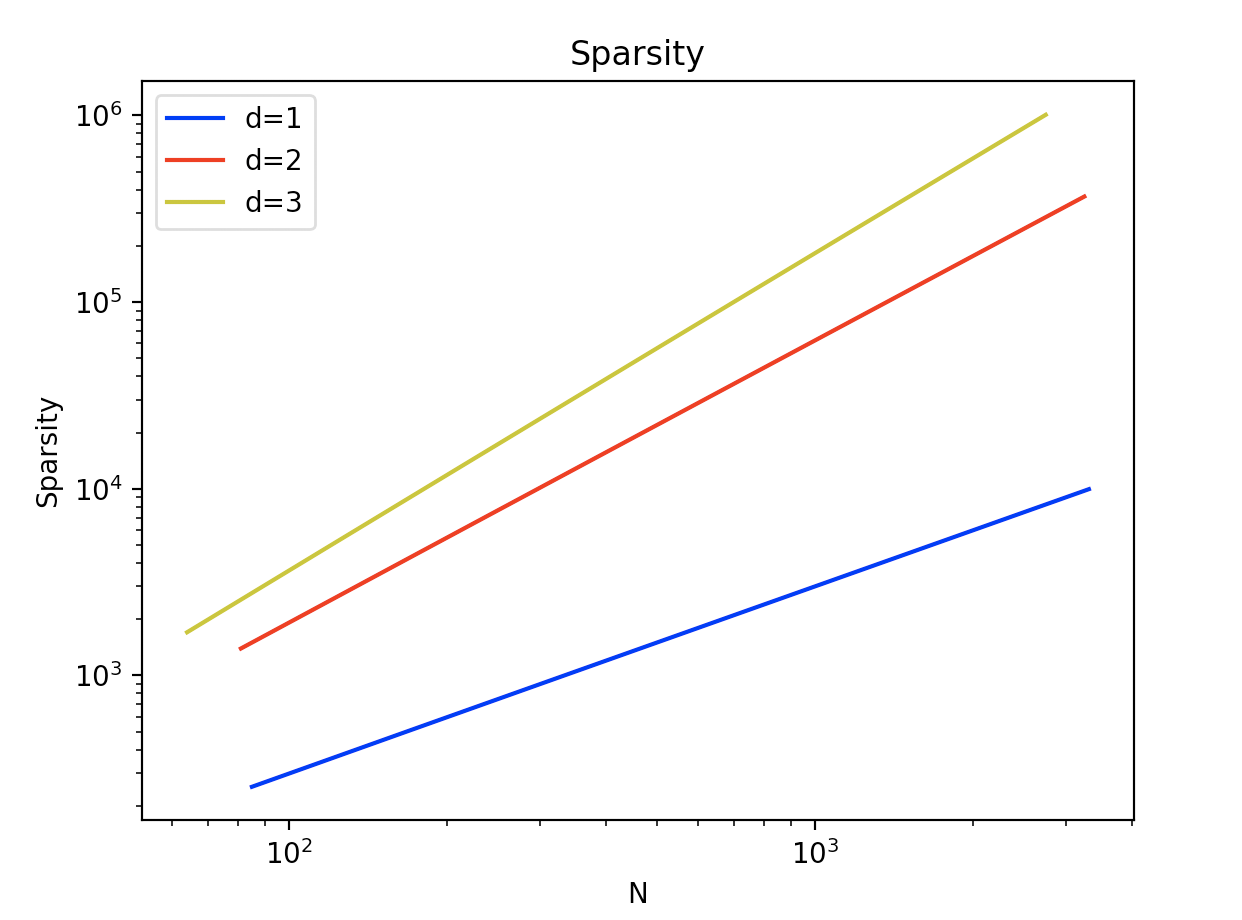
\includegraphics[scale = 0.6]{sparsity}
	\captionof{figure}{Sparsität der LU Zerlegung}
	\label{spar}

\end{minipage}
Auch hier ist zu erkennen, dass die Anzahl an Nicht-Null Einträgen exponentiell wächst, allerdings ist im Gegensatz zu der Kondition, welche wir uns oben angeschaut haben, die Steigung von der gelben Gerade, also in der dritten Dimension größer als in niedrigeren Dimensionen. Auch die  Anzahl an Nicht-Null Einträgen der Blockmatrizen wächst exponentiell, aber mit einer geringeren Steigerung. DIe Blockmatrizen sind also dünnbesetzter als die $LU$ Zerlegung dieser Matrix.


\section{Auswertung der Experimente}

Schaut man sich den Fehlergraphen an, so sollte man beachten, dass der Fehler sich aus dem Approximationsfehler und der Fortpflanzung des Rundungsfehlers. Bei der Fortpflanzung des Rundungsfehlers gibt die Kondition der Blockmatrix $A$ ein Maß an, wie stark sich der Fehler fortpflanzt. Bei großen Blockmatrizen ist dann der Approximationsfehler kleiner, da die Lösung an mehr Stützsteklen berechnet wird, aber dafür steigt die Kondition mit der Anzahl an Diskretisierungspunkten. Es lässt sich so erklären, warum die Fehler mit zunehmenden $N$ zunächst stark fällt, die Kondition ist noch nicht sehr groß und somit spielt die Fortpflanzung des Rundungsfehlers noch nicht so eine große Rolle. Dennoch wird die Approximation exakter und der Fehler insgesamt fällt. Später spielt der Rundungsfehler aufgrund von größerer Kondition eine entscheidende Rolle und so fällt der Fehler trotz zunehmender Genauigkeit der Approximation nicht mehr so stark.

Den Effekt von der Fortpflanzung des Rundungsfehlers haben wir genauer in der ersten Dimension untersucht. In der Abbildung \ref{conderror} ist zu erkennen, dass ein Rundungsfehler der Größe $10^{-3}r$ in der rechten Seite $f$ einen erheblichen Fehler in der Lösung des Approximationsproblem macht. Die Kondition der Blockmatrix der Größe $199$ beträgt $19999.99999999993$. Der fortgepflanzte Fehler ist also von der Größenordnung $19999.99999999993\cdot 10^{-3}r$. 

Wir haben gesehen, dass die Kondition von $A$ in der ersten Dimension am größten ist und am stärksten steigt. Das erklärt, warum der Fehler in dere ersten Dimension am höchsten ist und nur sehr langsam fällt. In der dritten dimension, steigt die Konditon nur langsam an, der Fehler fällt voarllem am Anfang sehr stark. Erst sehr spät fällt der Fehler nicht mehr so stark. Es fällt außerdem auf, dass wenn $n$  ein Teiler von $\kappa$ ist, der Fehler der Approximation sehr klein ist. Das liegt daran, dass die STützstellen dann genau auf den Nullstellen der Funktion liegen, und daher die approximierte Funktion an den Stützstellen nicht so stark abweicht.

Hilbert Matrizen sind besonders schlecht konditioniert. Besonders in der dritten Dimension erkennt man einen erheblichen Unterschied zwischen der Kondition der Blockmatrix und der hilbertmatrix der entsprechden Größe. 

In Abbildung \ref{graph()} und \ref{3d} erkennt man, dass mit größerem $n$, die approximierte Lösung schon viel näher an der exakten Lösung ist. Variiert man das $\kappa$, so fällt auf, dass eine Approximation mit $n<\kappa$ sehr schlecht sind, da sie die Struktur der Funktion noch gar nicht widerspiegeln.  Dies erkennt man auch in der Abbildung \ref{bigkappa}.

\section{Zusammenfassung}

Wir haben uns in diesem Bericht mit dem numerischen Lösen des Poisson Problems befasst. Dazu haben wir uns zunächstz überlegt, das Gebiet, auf dem das Problem gegeben ist, in unserem Fall $\Omega =(0,1)^d$ mit einem Gitter zu diskretisieren. Die Feinheit dieser Diskretisierung ist gegeben durch $n$, der Anzahl an Teilintervalle, in das wir $(0,1)$ zerlegen, um ein Gitter zu erhalten. Das Problem wird dann an $N=(n-1)^d$ Punkten diskretisiert. Somit erhalten wir nach Festlegung einer Ordnung auf den Diskretisierungspunkten durch Anwendung der Finiten Differnzen zur Diskretisierung des Laplace Operators, eine Blockmatrix $A$ der Größe $N\times N$. Setzen wir die Punkte in gegebener Reihenfolge in die Funktion $f$ ein, so erhalten wir einen Vektor $b$, sodass das Lineare Gleichungssystem $Ax=b$, welches das Poisson Problem löst. Um das lineare Gleichungssystem numerisch zu lösen, haben wir gesehen, dass man jede reguläre Matrix als Produkt $PLU$ schreiben kann, wobei $P$ eine Permutationsmatrix ist, $L$ eine linke untere Dreiecksmatrix und $U$ eine rechte obere Dreiecksmatrix ist. Durch diese $LU$ Zerlegung können wir dann durch Rückwärts und Vorwärtseinsetzen das Gleichungssytem vergleichsweise einfach lösen. 

Wir haben uns dann mit dem Fehler, der Sparsität und der Kondition der Blockmatrix mit zunehmender Anzahl an Diskretisierungspunkten $N$ angeschaut. Das haben wir jeweils für $d\in\{1,2,3\}$ getan. Wir haben einen Zusammenhang zwischen der Kondition der Blockmatrix und dem Fehler der Approximierten Lösung gefunden. Es ließ sich erklären, das der Fehler der Lösung sich aus dem Approximationsfehler und der Fortpflanzung des Rundungsfehlers zusammensetzt. Wie sehr sich der Fehler fortpfalnzt, lässt sich durch die Kondition beschreiben. Mit großem $N$ wird also zwar die Approximation genauer, allerdings die Kondition größer und somit auch die Fortplanzung des Rundungsfehlers. Wir haben uns außerdem die Sparsität der $LU$ Zerlegung angeschaut und diese mit der Sparsität der Blockmatrix verglichen. Es ist aufgefallen, dass die Anzahl an Nicht-Null EInträgen in der $LU$ Zerlegung weniger sind, diese also weniger dünnbesetzt sind als die Blockmatrizen.

\newpage
\section{Anhang}
\subsection*{Beschreibung der Implementierung}
Wir wollen später Gleichungssysteme mithilfe der LU-Zerlegung lösen und  dann \textit{Kondition}, die Anzahl der Nicht-Null-Einträge und den Fehler der Approximation im Vergleich zur exakten Lösung in unseren Experimenten genauer betrachten.
Hierzu haben wir drei Programme implementiert:

\subsection{\texttt{block\_matrix.py}}
Für unsere Blockmatrizen interessiert uns deren LU-Zerlegung, außerdem möchten wir in unseren Experimenten die \textit{Kondition} und \textit{Sparsity} vergleichen können.
Deshalb haben wir die Klasse \texttt{BlockMatrix} des Programms
\texttt{block\_matrix.py} um die folgenden Funktionen erweitert:

\subsubsection*{\texttt{get\_lu()}:}
Diese Funktion zerlegt unsere Matrix in eine orthogonale Matrix zur \textit{Pivorisierung}, eine untere linke Dreiecksmatrix mit Einsen auf der Hauptdiagonalen und eine obere rechte Dreiecksmatrix.
Wir verwenden dafür zunächst \texttt{get\_sparse()} um die Matrix zu erhalten, welche die entsprechende Dimension und Intervallzahl pro Dimension repräsentiert. Mit \texttt{todense()} ändern wir die Matrix in ein \textit{Numpy-Array}, sodass wir dann \texttt{scipy.linalg.lu()} verwenden können. Das liefert uns schon das Erwünschte.

\subsubsection*{\texttt{eval\_sparsity\_lu()}:}
\texttt{eval\_sparsity\_lu()} soll die absolute Anzahl an Nicht-Null-Einträgen der \textit{LU-Zerlegung} einer Matrix, sowie die relative Anzahl ausgeben. 
Es muss also zuerst die \textit{LU-Zerlegung} bestimmt werden. Hierfür können wir \texttt{get\_lu()} verwenden. Die Nicht-Null-Einträge von $L$ und $U$ lassen sich durch \texttt{numpy.count\_nonzero()} ermitteln. Um die absolute Anzahl zu erhalten addieren wir die beiden Werte, ziehen aber noch $(n-1)^d$ ab, denn wir möchten die Einsen auf der Hauptdiagonalen nicht mitzählen.
Der relative Wert berechnet sich dann, indem wir die absolute Anzahl durch die Zahl an Elementen der Koeffizientenmatrix ($=(n-1)^{2d}$) teilen.

\subsubsection*{\texttt{get\_cond()}:}
\texttt{get\_sparse()} bringt uns unsere Koeffizientenmatrix. Die \textit{Kondition} berechnet sich dann mit folgender Formel:
$$
cond(A)=||A^{-1}||_{\infty}||A||_{\infty}
$$
Die Bestimmung der Inversen und der Norm erfolgt mithilfe von 
\texttt{scipy.sparse.linalg}-Funktionen.



\subsection{\texttt{linear\_solvers.py}}
Mit diesem Programm kann man Gleichungen der Form $Ax=b$ lösen. Dies geschieht über eine \texttt{pivotisierte LU-Zerlegung}.

\subsubsection*{\texttt{solve\_lu()}:}
Diese Funktion benötigt als Input $p , l , u$ und $b$ und gibt uns die Lösung $x$ des Gleichungssystems wieder.
Wir können die Dreiecksform unserer Matrizen ausnutzen und $x$ durch \textit{Vorwärts- und Rückwertseinsetzen} bestimmen. Das Ganze wird dann durch \texttt{scipy.linalg.solve\_triangular()} umgesetzt.
Wir bestimmen zunächst $y$ aus
$$
Ly = P^{-1}b
$$
Da $P^{-1}$ eine orthogonale Matrix ist, können wir \texttt{numpy.transpose(p)} nutzen.
Im zweiten Schritt liefert uns
$$
Ux=y
$$
unsere Lösung $x$.

\subsection{\texttt{poisson\_problem.py}}
Wir wollen den Fehler der Approximation im Vergleich zur exakten Lösung vergleichen können. Dieses Programm erweitern wir deshalb um folgende Funktion:

\subsubsection*{\texttt{compute\_error()}:}
Hier wird der maximale absolute Fehler der Approximation an den Diskretisierungspunkten berechnet, bezüglich der \textit{Infinity-Norm}. Dazu nimmt die Funktion als Input die Dimension, die Anzahl an Intervallen pro Dimension, die exakte Lösung des \textit{Poisson-Problems} an den Diskretisierungspunkten und die Funktion welche das \textit{Poisson-Problem} löst.
Dafür gehen wir sukzessive die Diskretisierungspunkte durch, bestimmen dessen Koordinaten mithilfe von \texttt{inv\_idx} und erhalten mit $u(x)$ die exakte Lösung. 
Die \texttt{Infinity-Norm} der Differenz zur Approximierten Lösung gibt uns dann unseren Wert für den Fehler.

\section{Zusätzliche Grafiken}
\begin{minipage}{\textwidth}

 \centering
 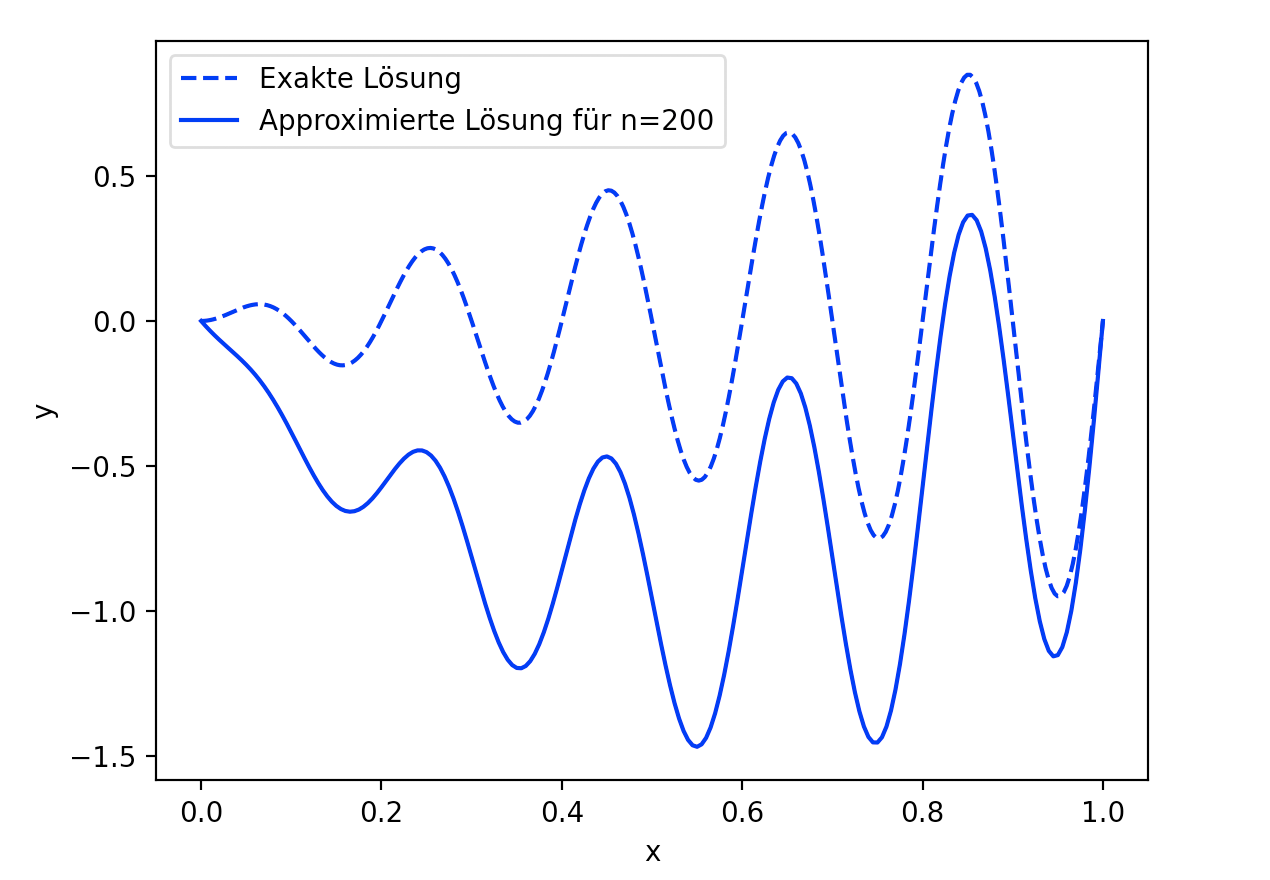
\includegraphics[scale = 0.6]{kondition_Fehler}
 	\captionof{figure}{Fortpflanzung eines Rundungsfehlers}
 	\label{conderror}
\end{minipage}




\begin{minipage}{\textwidth}
\centering
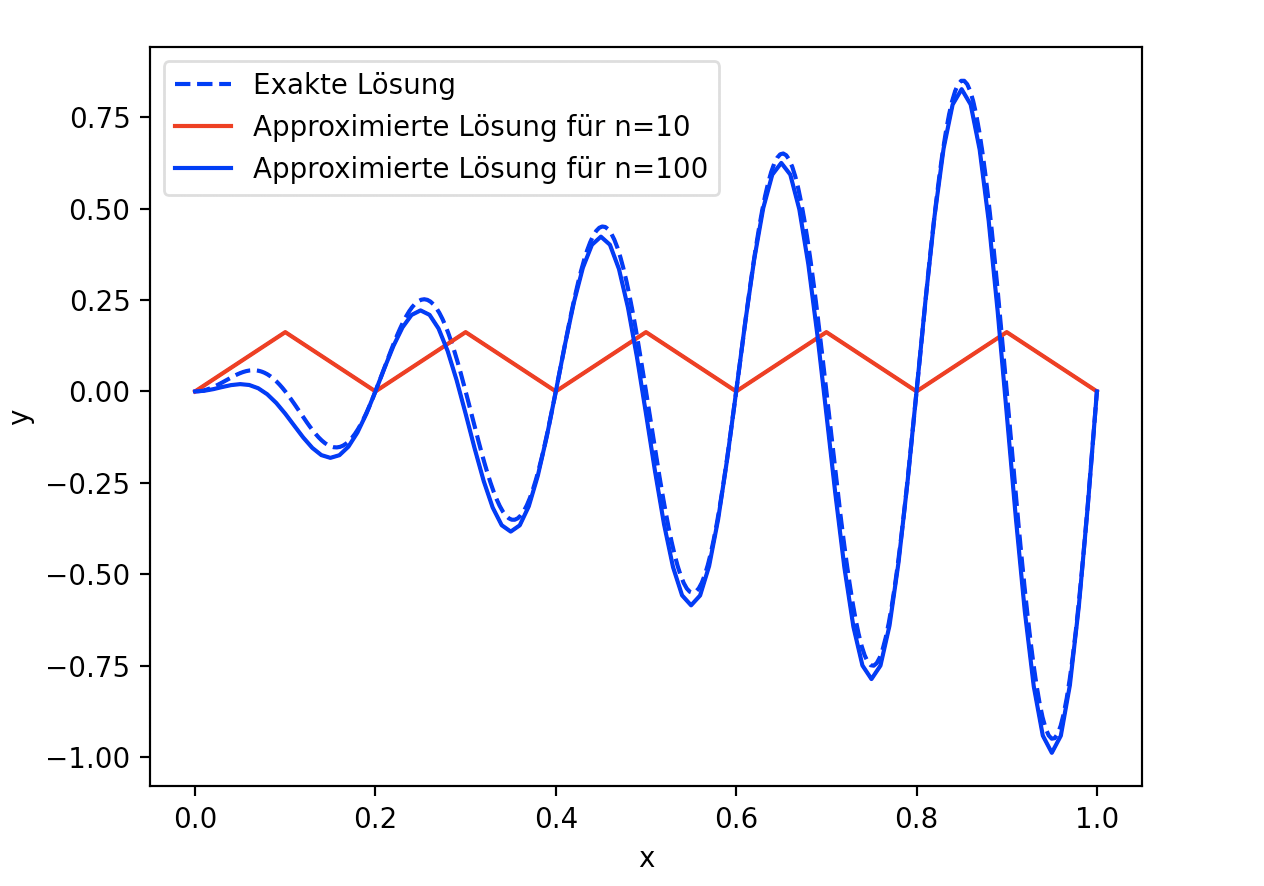
\includegraphics[scale = 0.60]{graph().png}
    \captionof{figure}{Vergleich exakte und approximierte Lösung für $d=1$, $\kappa =6$}
    	\label{graph()}
\end{minipage}



\begin{minipage}{\textwidth}
\centering
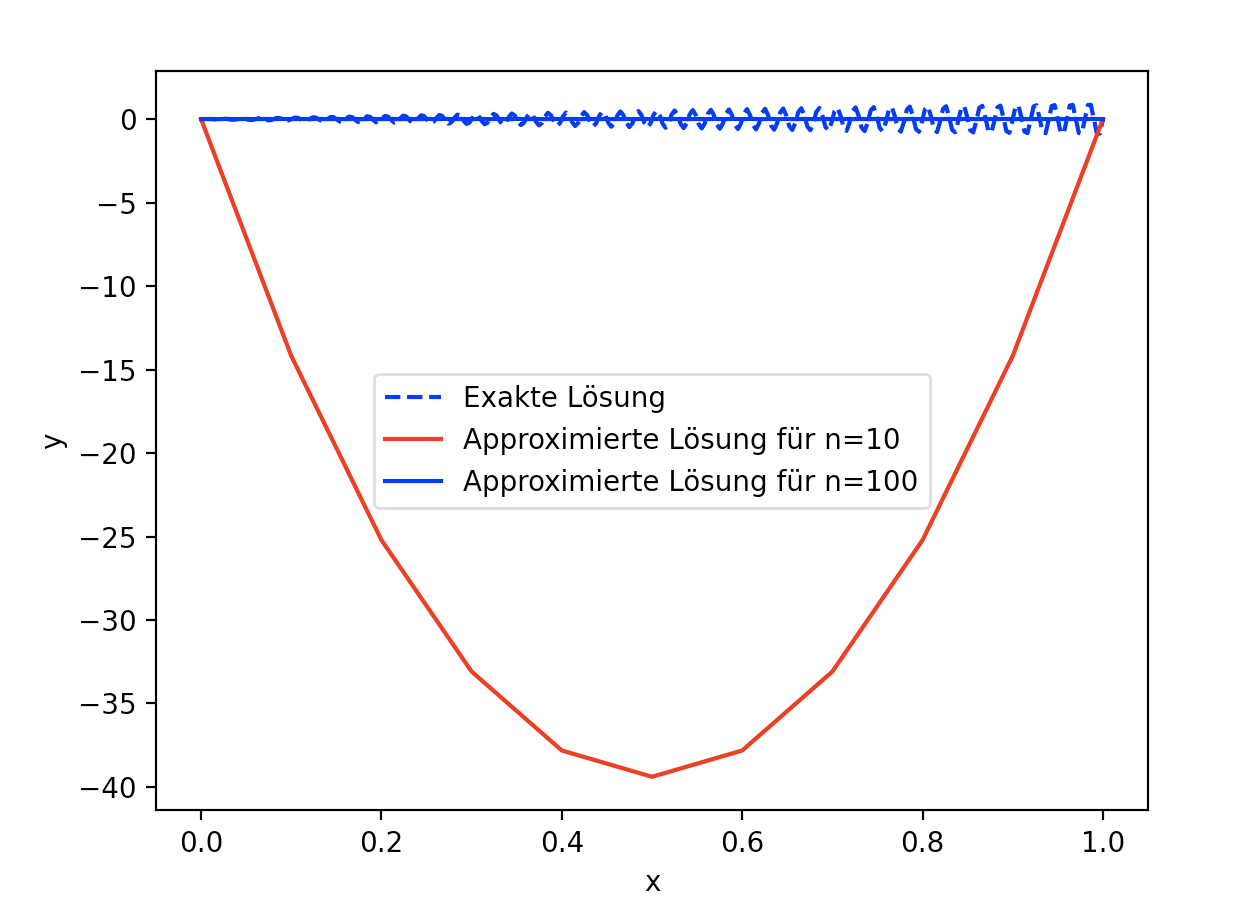
\includegraphics[scale = 0.60]{bigkappa}
    \captionof{figure}{Vergleich exakte und approximierte Lösung für $d=1$, $\kappa =100$}
    	\label{bigkappa}
\end{minipage}




\printbibliography

%%% END OF DOCUMENT %%%%%%%%%%%%%%%%%%%%%%%%%%%%%%%%%%%%%%%%%%%%%%%%%%%%%%%%%%%
\end{document}
